\cleardoublestylepage{common}

\newcommand{\paragraphnl}[1]{\paragraph{#1}\hspace{0pt}\\}

\section{正文}

\subsection{目标}

本部分描述本设计所开发的系统的功能与目的。

\subsubsection{背景与趋势}

本设计的题目来源于真实世界中的现状,在互联网应用和服务中,随着产业日趋完善,很多同类型,同质的应用程序将会日趋集中化部署。这一现象的推动者包括云服务,无论公有云或是私有云,也包括大企业的平台化,中台化发展方式。其好处包括降低应用使用者自行维护的心理负担,而平台方可以投入更多精力优化,且统一部署能提供更多的优化空间。例如考虑不同租户之间的亲和性等等。

对于大规模在线服务应用的资源调度解决方案这样一个题目来说,范围未免太宽泛了,本设计选择以基于 Tensorflow Serving 的机器学习在线服务为范例,考虑各个机器学习模型的性能要求,资源要求等特性,将其编排并部署到工业生产级别的调度系统中。以此为例来研究并给出一套解决方案。

% \subsubsection{问题与解决方案}

\subsection{开发技术}

本部分列出工程实现上所依赖的全部技术。

golang v1.11.5

GoLand 2019.1.1

Kubernetes v1.14

minikube 1.0.0

operator-framework v1.0.0

\subsection{工程背景}

本部分将会论述为了实现本系统,依赖的开源组件与开源解决方案等。

\subsubsection{Kubernetes}

Kubernetes \cite{kubernetes} (下文中可能简称为k8s)是由云原生基金会所维护的项目,其设计思想脱胎于 Google 内部使用的 Borg 集群管理系统 \cite{borg} 。Kubernetes 借助于容器的实现,负责容器编排与资源调度分配,其作用与 Apache Hadoop YARN \cite{hadoop} 类似。Kubernetes 的概念与所包含的组件在下文中详细介绍,通过这段说明可以使读者更容易理解如此一个容器编排系统负责了什么工作,解决了什么问题。

\subsubsection{Tensorflow Serving}

Tensorflow 是近年来生态最完善的深度学习框架之一,从其工作方式来看,也可以被称为计算图框架。其深度学习相关的部分我们不在这里做过多讨论,有很丰富的资料,感兴趣的读者可以自行查阅。这里我们介绍一下 Tensorflow Serving \cite{serving} ,这个负责使用训练好的模型的组件,其工作方式,与容器生态的关系,最终得出为何用它作为本设计中的代表应用的例子。

Tensorflow Serving 可以将 Tensorflow 训练得到的模型,注意默认支持 saved model 格式的模型,对 tensorflow 产出训练结果有了解的读者应当知道其中差别。

用户运行 Tensorflow Serving 时,通过命令行参数或者环境变量等等方式传递模型的名称,路径等参数,不需要修改源代码或者编写更多的代码就可以使模型上线服务,这样可以做到模型数据和逻辑的分离,对方便使用,加快部署迭代速度有帮助。

Tensorflow Serving 非常注重面向容器的生态,不难得出结论,只需提供模型的数据文件,就可以被加载服务,这说明 Tensorflow Serving 属于带数据的只读服务。结果上,Tensorflow Serving 官方将 docker image 作为比二进制更重要的发布渠道,用户通过 docker registry pull 合适版本的 Serving 镜像,就可以直接使用,无疑是更方便运维,对比与使用的。这也是我选择使用 Tensorflow Serving 作为示例应用,进行对它的调度算法实验,开发的重要原因。另一个重要原因是,作为机器学习服务,它属于业务逻辑和框架本身界限明显,明确区分,分开理解的典型代表。如果从数据/业务与框架分离的角度考虑,任何一个区分租户的数据库或搜索引擎系统也可以作为例子,但是这里他们的代表性不如机器学习服务明显,且机器学习作为相对而言的新兴事物,对它的尝试和探索更有价值。但是这不代表本设计的成果就对其他领域没有意义了,这一点还需要读者明辨。

\subsubsection{Kubernetes Operator}

Kubernetes Operator \cite{operator} 是 Kubernetes 生态中为用户自己提供调度逻辑和功能扩展的一类接口与实现方式的总称。

\subsection{实现方式}

本部分将会详细讲解本人实现此系统的详细过程。最终完成的系统概貌如图 \ref{fig:system} 所示。

\begin{figure}

\centering

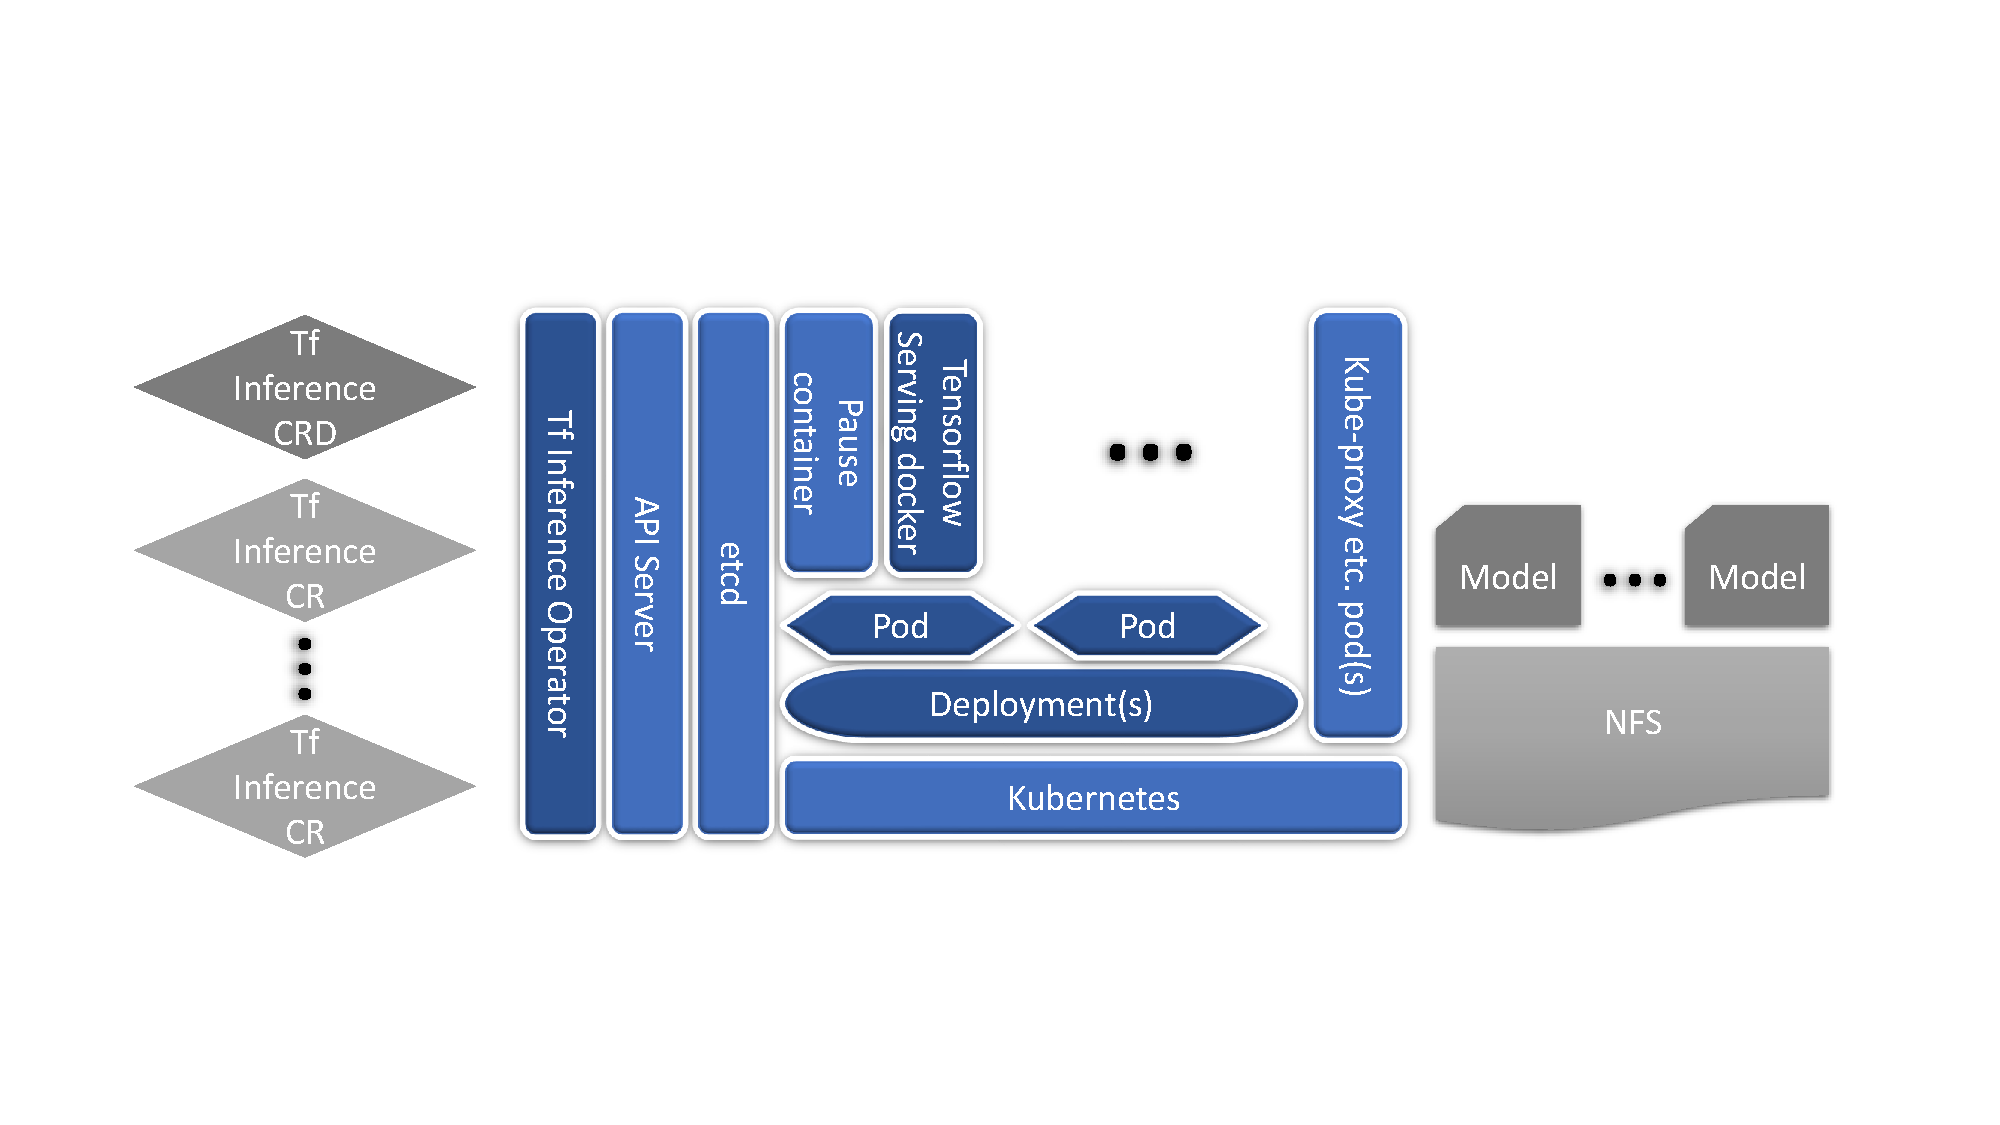
\includegraphics[width=0.8\textwidth]{system-pic.pdf}

\caption{系统概要}\label{fig:system}

\end{figure}

\subsubsection{搭建 Kubernetes 开发环境}

作为一个生产级别的容器编排系统,天然就是面向分布式系统,保证可靠性的,工作方式也需要天然面向分布式系统,为部署在多台机器上做设计。同时此系统将应用程序的运行,甚至网络环境都进行了接管,因此对运行环境有很强的依赖。实际操作上也是如此,我调研了多种搭建 Kubernetes 环境的方案,最终只有一种方式实现起来相对简单。下面概要讲解一下各种搭建方式的优劣,以及我最后的选择。

\paragraphnl{Kernel and Services Requirements}

本部分讲解运行 Kubernetes 的机器需要满足的条件。

Kubernetes 本身需要在 Linux 服务器上运行,而 Kubernetes 本身是否运行在虚拟机当中又造成了环境需求的不一致。不过总的来讲,我们的开发环境需要满足以下这些需求就能够运行。对于内核来说,需要支持 iptables 的大部分调度算法类内核模块,以便支持 Kubernetes 网络相关的功能。需要支持 KVM,以便我们选择 KVM 作为运行 minikube 虚拟机的后端,同时需要支持 libvirt 需要的部分功能。我们还可能需要多种内核 namespace 支持,包括 mount namespace, pid namespace 等等,以及部分文件开关和杂项以便支持 docker 工作。好在编译安装 docker 与 libvirt 时,脚本会对内核选项进行校验,并输出不满足的项目。最后我们还需要 NFS 支持,如果需要像我一样使用 NFS 挂载模型数据目录的话。

这里我们假设读者有能力自行配置内核编译选项,并且编译安装内核。较为成熟的发行版往往会提供发行版官方分支的内核源码软件包供我们使用。并且我们这里要求的内核功能在主流发行版当中往往是默认开启的,这里的介绍涉及一些原理,给读者补充背景知识并且留作备用。

至于内核之外的软件包和服务,我们需要按需安装并调通 docker, libvirt, qemu-kvm 等,视用户打算采用本机方式安装或者虚拟化方式安装而定。

\paragraphnl{DinD approach}

DinD 指代 Docker in Docker。这是一种单机部署 Kubernetes 测试集群的方案,并且有人已经在 Github 上开源了一整套工具脚本和解决方案。这一方案适合于用户有能运行 Docker 的 Linux 主机,但是没有虚拟化能力。对于具有对主机的完全控制力和虚拟化能力的情况来讲,DinD 方案也可以采用,但表现不一定有官方性质维护的 minikube 效果更好,在 troubleshooting 和资料支持方面。

在此方案下,我们使用一个功能类似于 minikube 的虚拟机的 Docker 镜像,作为运行 kubernetes 集群的主机,在这个容器内运行 Kubernetes 组件的容器。这样带来的一个问题是,需要宿主机内核完全支持 kubernetes 运行需要的一切特性,且隔离程度不够,docker 版本也需要和 kubernetes 可以配合。

本人的尝试当中,DinD 镜像与容器可以启动,但是工作不完全正常,内部有 kubernetes 组件报错,最终在考量了成本和收益之后,本人选择放弃使用这个方案。

\paragraphnl{Bare Metal approach}

Bare Metal 可以翻译为裸金属服务器,指没有经过任何虚拟化的裸机。这里本人使用个人电脑上安装的 gentoo Linux,读者复现此方案时需要一台任意的 Linux 计算机。Kubernetes 官方网站上存在所有组件的说明和配置方式,也有第三方文档详细描述这里的细节问题,如域名和证书配置,网络方案的选择与配置等细节。

本人出于逐步研究 kubernetes 核心组件的目的,在裸机上配置了 kubernetes 的大多数组件,最后也没有完全完成这些配置。因为这些内容工作量极大并且和本设计的重心无关。达到了了解系统的部署方式这一目标之后就没必要继续了。

% TODO: links

\paragraphnl{minikube local approach}

minikube 是 kubernetes 团队官方提供的一个用于快速部署单机测试集群的工具,其支持所有主流操作系统。事实上,minikube 同时支持 Windows,macOS,Linux 三大平台,因为主要运行在虚拟机中,系统本机的操作系统环境本身不被依赖。几乎所有主流的虚拟机都被支持,包括了 KVM, VirtualBox, HyperV, VMWare Fusion 等。

在一些基本的配置正确的情况下,minikube 可能是最容易成功运行的方式。尽管如此,这个所谓的“开箱即用”也需要环境满足一些基本要求,例如某些平台下,可以运行 docker-machine。

因为虚拟机后端可以被任意替换,minikube 支持将后端配置为 none 从而支持将宿主机直接作为“虚拟机”来使用。这样会对你的宿主机环境添加两个额外的要求:一、你的宿主机需要可用的 docker 服务;二、你需要使用 root 权限运行从而允许 minikube 向宿主系统中安装程序。

此模式的好处是减少了虚拟机的性能开销,且更容易访问运行 kubernetes 的环境,但是对本机的污染和依赖是需要我们付出的代价。

\paragraphnl{minikube VM approach}

这里我们使用一种虚拟机作为后端来启动 minikube 的单机 kubernetes 集群。Linux 平台上的默认选择是 VirtualBox,作为一个开源且免费的优秀虚拟机管理软件,因为优异的跨平台性能被作为了 minikube 在多个平台上的默认的虚拟机后端。但是这里我们选择更加 Linux 友好,功能更强的 KVM 作为后端,进行一次配置尝试。KVM 全名为 Kernel-based Virtual Machine,正如其名,是 Linux 内核支持的虚拟机 Hypervisor。正如上文中描述过,若使用此方式,需要配置内核支持 KVM 的开关。因为内核和 Hypervisor 二合一,效率会更高。同时这也是工业界和云服务提供商常用的虚拟化方式,经受住了考验,因此这里我们选择 KVM 进行实验。

下面我们给出此方式运行 kubernetes 集群的命令与输出,方便读者理解此工具都执行了哪些任务。

\begin{lstlisting}[language=bash]

sudo minikube config set vm-driver kvm2
sudo minikube start

\end{lstlisting}

若一切顺利,minikube 正常执行了一切任务,应当见到与下述类似的输出内容。

\begin{lstlisting}[language=bash]
🐳  Version of container runtime is 18.09.2
⌛  Waiting for image downloads to complete ...
E0424 00:19:35.003745    1889 start.go:209] Error caching images:  Caching images for kubeadm: caching images: caching image /root/.minikube/cache/images/gcr.io/k8s-minikube/storage-provisioner_v1.8.1: fetching remote image: Get https://gcr.io/v2/: dial tcp 74.125.204.82:443: i/o timeout
✨  Preparing Kubernetes environment ...
❌  Unable to load cached images: loading cached images: loading image /root/.minikube/cache/images/gcr.io/k8s-minikube/storage-provisioner_v1.8.1: stat /root/.minikube/cache/images/gcr.io/k8s-minikube/storage-provisioner_v1.8.1: no such file or directory
🚜  Pulling images required by Kubernetes v1.14.0 ...
🚀  Launching Kubernetes v1.14.0 using kubeadm ... 
⌛  Waiting for pods: apiserver proxy etcd scheduler controller dns
🔑  Configuring cluster permissions ...
🤔  Verifying component health .....
🤹  Configuring local host environment ...

⚠️  The 'none' driver provides limited isolation and may reduce system security and reliability.
⚠️  For more information, see:
👉  https://github.com/kubernetes/minikube/blob/master/docs/vmdriver-none.md

⚠️  kubectl and minikube configuration will be stored in /root
⚠️  To use kubectl or minikube commands as your own user, you may
⚠️  need to relocate them. For example, to overwrite your own settings:

    ▪ sudo mv /root/.kube /root/.minikube $HOME
    ▪ sudo chown -R $USER $HOME/.kube $HOME/.minikube

💡  This can also be done automatically by setting the env var CHANGE_MINIKUBE_NONE_USER=true
💗  kubectl is now configured to use "minikube"
🏄  Done! Thank you for using minikube!
\end{lstlisting}

下面给出集群启动之后所运行的 docker 容器列表。

\begin{lstlisting}
CONTAINER ID        IMAGE                  COMMAND                  CREATED             STATUS              PORTS               NAMES
5d416847c422        5cd54e388aba           "/usr/local/bin/kube…"   20 hours ago        Up 20 hours                             k8s_kube-proxy_kube-proxy-qtctj_kube-system_ba4c62f4-65e3-11e9-9acd-3a4feb33d13b_0
be34a9157d37        k8s.gcr.io/pause:3.1   "/pause"                 20 hours ago        Up 20 hours                             k8s_POD_kube-proxy-qtctj_kube-system_ba4c62f4-65e3-11e9-9acd-3a4feb33d13b_0
6c0e3702a706        k8s.gcr.io/pause:3.1   "/pause"                 20 hours ago        Up 20 hours                             k8s_POD_coredns-fb8b8dccf-tfct6_kube-system_ba4c6fa2-65e3-11e9-9acd-3a4feb33d13b_0
46fb09b54279        k8s.gcr.io/pause:3.1   "/pause"                 20 hours ago        Up 20 hours                             k8s_POD_coredns-fb8b8dccf-ssr52_kube-system_ba4bc787-65e3-11e9-9acd-3a4feb33d13b_0
fde495430bdf        k8s.gcr.io/pause:3.1   "/pause"                 20 hours ago        Up 20 hours                             k8s_POD_storage-provisioner_kube-system_ba4780d4-65e3-11e9-9acd-3a4feb33d13b_0
05e94c674ce5        00638a24688b           "kube-scheduler --bi…"   20 hours ago        Up 20 hours                             k8s_kube-scheduler_kube-scheduler-minikube_kube-system_58272442e226c838b193bbba4c44091e_0
0e0f32af6c4b        ecf910f40d6e           "kube-apiserver --ad…"   20 hours ago        Up 20 hours                             k8s_kube-apiserver_kube-apiserver-minikube_kube-system_267a4c5b83c2f08d16cd0b2fb496fdf3_0
59a4d5ce55c5        2c4adeb21b4f           "etcd --advertise-cl…"   20 hours ago        Up 20 hours                             k8s_etcd_etcd-minikube_kube-system_973c2fad42d1ca0c0cafe14fa28f9a70_0
ad0edb256af6        b95b1efa0436           "kube-controller-man…"   20 hours ago        Up 20 hours                             k8s_kube-controller-manager_kube-controller-manager-minikube_kube-system_6f22129755f0edc1e35623595e40aab2_0
cf7beb5a9f2b        119701e77cbc           "/opt/kube-addons.sh"    20 hours ago        Up 20 hours                             k8s_kube-addon-manager_kube-addon-manager-minikube_kube-system_0abcb7a1f0c9c0ebc9ec348ffdfb220c_0
218f0881a76a        k8s.gcr.io/pause:3.1   "/pause"                 20 hours ago        Up 20 hours                             k8s_POD_kube-scheduler-minikube_kube-system_58272442e226c838b193bbba4c44091e_0
b04d338f0290        k8s.gcr.io/pause:3.1   "/pause"                 20 hours ago        Up 20 hours                             k8s_POD_kube-apiserver-minikube_kube-system_267a4c5b83c2f08d16cd0b2fb496fdf3_0
f7a634bc0085        k8s.gcr.io/pause:3.1   "/pause"                 20 hours ago        Up 20 hours                             k8s_POD_kube-controller-manager-minikube_kube-system_6f22129755f0edc1e35623595e40aab2_0
446a4cd0e374        k8s.gcr.io/pause:3.1   "/pause"                 20 hours ago        Up 20 hours                             k8s_POD_kube-addon-manager-minikube_kube-system_0abcb7a1f0c9c0ebc9ec348ffdfb220c_0
e4d548c62aa5        k8s.gcr.io/pause:3.1   "/pause"                 20 hours ago        Up 20 hours                             k8s_POD_etcd-minikube_kube-system_973c2fad42d1ca0c0cafe14fa28f9a70_0
\end{lstlisting}

\subsubsection{搭建 Kubernetes Operator 开发环境}

在可以连接并管理一个 Kubernetes 集群的前提下,我们可以开发自己的 Operator,并且以某些方式运行我们的 Operator,让它进行决策,并且向 API Server 提交 API 对象以执行我们需要的行为。

Operator Framework 支持包括 golang,Ansible 在内的几种编程语言或工具。这其中 golang 由于靠近 docker,云原生等生态系统,一定会提供,Ansible 架构则是传统集群管理自动化运维的工具,主要推动方是 Redhat,出现在这里也很合乎习惯。为了贴近生态,更容易在 troubleshooting 时获取信息,也为了通用编程语言处理逻辑时的便捷性,本人选择 golang 作为开发语言。

Operator Framework 可以理解为是一套 golang 语言开发的,提供 Operator 基本功能的库。它包装了 leader 选举,程序入口,常用操作 utils 等内容。我们编写的 Operator 逻辑可以在依赖,扩展 Framework 提供的代码的基础上进行。

Operator SDK 是一个命令行工具。上述框架代码的很多细节,手工编写意义不大且容易出错,SDK CLI 可以帮助我们生成。同时当我们为自己的 Operator 添加功能模块时,编写了部分抽象定义的代码,SDK 帮助我们以代码生成的方式生成模版代码,被内部其他逻辑使用。最后,我们编写的代码如果要在 Kubernetes 集群中运行,需要相对而言繁琐一些的编译,构建,制作 docker 镜像等发布流程,而 SDK CLI 可以帮助我们一键式在集群外运行 Operator,与集群交互,极大加快了迭代测试的速度。

下面给出使用 Operator-SDK 时,常用的几个操作如何执行,也方便读者理解系统运行的方式,从而理解本文内容。

%TODO: stdout

\subsubsection{开发调度执行模块}

定义 CRD 与 CR,CRD 为自定义资源定义,给出了我们添加的自定义资源的模板,CR 为自定义资源,是这种定义下的一个实例。利用 OOP 的概念来解释的话,CRD 就是类型 class,CR 就是实例 instance。下面给出本人编写的 yaml 格式的定义以及对应的 golang 数据结构,再解释其释义。

下面是 golang 编写的数据结构定义,不重要的代码,空行和注释已经略去。可见我们将调度的信息输入写入了定义中,用户只要提交任务时照原样写好定义即可使用。

\begin{lstlisting}[language=go]

// Added by Zhenyun Yu, types here are necessary for specs
type Model struct {
    Name string `json:"name"`
    Memory int32 `json:"memory"`  // in MB
    ComputingResource int32 `json:"computing\_resource"`  // 100 for each core
}

type Node struct {
    Memory int32 `json:"memory"`
    ComputingResource int32 `json:"computing\_resource"`
}

// TfInferenceSpec defines the desired state of TfInference
// +k8s:openapi-gen=true
type TfInferenceSpec struct {
    Models []Model `json:"models"`
    Nodes []Node `json:"nodes"`
}

type TfInferenceStatus struct {
    Deployments []string `json:"deployments"`
}

type TfInference struct {
    metav1.TypeMeta   `json:",inline"`
    metav1.ObjectMeta `json:"metadata,omitempty"`

    Spec   TfInferenceSpec   `json:"spec,omitempty"`
    Status TfInferenceStatus `json:"status,omitempty"`
}

// TfInferenceList contains a list of TfInference
type TfInferenceList struct {
    metav1.TypeMeta `json:",inline"`
    metav1.ListMeta `json:"metadata,omitempty"`
    Items           []TfInference `json:"items"`
}
    
\end{lstlisting}

下面给出的是 yaml 格式的 CRD 定义去除不重要的部分后的结果,可见它是对所有 CRD 类型的抽象,仅给出了名字,版本等元数据,与内容关联不大。事实上我们也仅依靠他“注册”类型,而不依赖具体内容。

\begin{lstlisting}

    apiVersion: apiextensions.k8s.io/v1beta1
    kind: CustomResourceDefinition
    metadata:
      name: tfinferences.serving.example.com
    spec:
      group: serving.example.com
      versions:
      - name: v1
        served: true
        storage: true

\end{lstlisting}

\subsubsection{开发算法实现}

由上下文给出的分析可知,我们的调度算法是一个纯函数,在给定业务模型定义和服务器节点资源定义后,输出一组编排方式,它的输入与输出都是给定的,下面我们把函数签名(golang 语法)给出:

\begin{lstlisting}

func getDeploymentMetas(models []servingv1.Model, nodes []servingv1.Node, groups []servingv1.Group) []DeploymentMeta

\end{lstlisting}

\subsubsection{联调测试}

本部分讲述本设计中在基本完成代码的开发与测试后,如何测试系统能否正常工作,观察效果以及使用方式。

我们可以先使系统运行,然后向其提交一个 CR 描述,随后观察 Operator 有没有执行,得到正确的部署。我们将提交的 CR 文件与测试结果附在下方。

\begin{lstlisting}

apiVersion: serving.example.com/v1
kind: TfInference
metadata:
  name: example-tfinference
spec:
  models:
    - name: mnist
      memory: 100
      computing_resource: 50
    - name: dummy
      memory: 50
      computing_resource: 10
  nodes:
    - memory: 1024
      computing_resource: 200

\end{lstlisting}

 % TODO: pic

% \subsubsection{结果对比}

% TODO: do what here?

\subsubsection{难点与问题}

本部分讲述在实现的过程当中,本人遇到了哪些难以解决的问题,最后又是如何克服的。这部分旨在让读者明白完成一个工程项目比起理论算法研究的不同之处,以及在实现的过程当中本人的时间和精力主要用于解决哪些问题了。

\paragraphnl{开发环境权限控制}

我们的部署可能需要 root 用户来访问 minikube 测试集群,而采用非特权用户来开发 Operator 程序。这样可以保证开发过程不会因为权限问题影响系统稳定性,但是调试,运行时难以互通。这里本人通过符号链接等方式同步两侧的环境,保证最终联调测试的环境可以工作。

\subsubsection{工程实现细节与亮点}

本部分讲述工程细节中的细节问题和自认为比较亮点的解决方案。

\paragraphnl{NFS 网络文件系统}

假设不采用任何分发数据的手段和设计,我们的工程就是空中楼阁,服务最终并不能自然且顺利地获得自己的模型数据,那么一切调度逻辑也就失去了意义。这里一般的做法是将模型数据打包进入镜像,这样的好处是应用启动之前随着镜像分发模型,应用启动之后不会再有性能和带宽的问题,但是也会影响迭代速度,每一次调度和堆叠都可能需要重新打包镜像,严重阻碍了实时性。因此,本设计中采用了应用和模型数据分离的方式来工作。

对于业务配置和数据,我们的场景下需要每一台服务器都可以访问,并且保证足够的性能。对于规模在数十到数百台服务器之间的服务器集群来讲,我们可以采用高速网络支撑的网络文件系统来分发数据。应用 pod 启动时,将独立于集群外的 NFS 目录挂载到需要的路径,应用按需读取数据时,通过网络实际分发文件数据。这种方式可以在中等规模的服务集群中提供及时的数据发布与更新服务,并且解除了 docker 镜像和服务配置逻辑,模型数据的强耦合。

\paragraphnl{嵌套虚拟化与局域网网络空间映射}

为了搭建这个环境,我的测试机本机与开发环境虚拟机之间使用虚拟网桥连接,可以互相通信。同时虚拟机之中的嵌套虚拟化 minikube 虚拟机也挂载了自己的虚拟网卡,桥接到外部网络上,这样各个计算机的网络就具有了平等的网络拓扑。平等拓扑的好处是各个机器之间可以互相访问,任意一处都可以访问 kubernetes 集群以测试集群工作状态,访问外部计算机方便我们部署数据与网络文件系统不受影响,交换数据方便等等。

\paragraphnl{编排算法至 Kubernetes Deployment 映射}

为了描述不同应用的部署,kubernetes 抽象出了多个概念。对于无状态,可以横向扩展的应用来讲,这个概念叫做 Deployment。我们的Operator 只需保证一个概念,即任意时刻,我们所需要在线服务中逻辑集群,都有对应的 Deployment 存在。如此 kubernetes 便可以帮我们将部署调节至目标状态。

但是我们的 Operator 所处理的一份用户输入,会被算法划分为多个逻辑集群,这需要我们的 Operator 同时维护多个 Deployments。如何维护我们的逻辑集群到 kubernetes deployment 对象的映射关系才方便?本设计的做法是,将唯一确定一个 deployment 信息的数据,包括模型和所有模型的硬性数据。将他们按照固定的算法排序后序列化作为键,再哈希为短十六进制字符串,作为 deployment 命名的一部分。这种设计下,deployment 的名称后将有短横线分隔的两个哈希值,分别代表 CRD 的键和逻辑集群的键,含义可以在调试时观察,也不会过长,且作为 Operator 操作的依据。

\subsection{算法描述}

本部分讨论在不涉及系统实现的细节前提下,调度算法的背景,意义与实现。

\subsubsection{背景}

本部分讨论一个通用的调度算法需要考虑哪些内容。

我们先思考一下,一个通用的应用程序运行需要依赖哪些资源。资源总共分为软件资源和硬件资源两类。软件资源包括操作系统版本,动态链接库依赖等,这里不在我们的主要讨论范围之内,暂时不考虑。硬件资源包括计算资源,即处理器时间;存储资源,包括主存储器,外置存储器如硬盘容量;网络带宽;异构计算设备,包括,型号,类型,使用率等等限制。

这里定义我们的调度算法为,在软件资源依赖能满足的前提下,将不同的多租户应用部分编排至不同的应用与机器,并保证满足各个租户业务与数据的资源声明得到满足。

为了满足这些资源限定,一个通用的算法需要对可能出现的所有资源类型进行分类,才能从更抽象的角度进行考虑。因为我们无法枚举可能出现的一切资源类型。

一切资源限度要求,都可以用一个标量来描述。如 CPU 计算资源需求,可以将单位核数输出的计算力定义为一个定值,假设就是 100,那么每个应用对 CPU 计算能力的要求就可以使用一个数值来描述了。抽象来讲,即是一个标量加上任意自定义的单位即可描述。

然而考虑到计算资源横向扩展的要求,资源的种类又需要做出区分。考虑内存消耗,对于深度学习模型而言,内存消耗主要是模型加载至内存中,每一台运行服务的服务器都需要消耗等量的内存。再考虑计算资源消耗,对于稳定相同的计算任务或者流量,消耗的总计算力之和不变,横向扩展后新增的服务器不需要额外浪费计算力,而是负担了原有服务器不能承担的一部分任务。我们将前一种横向扩展后每台服务器都要消耗等量的资源称为硬性资源,后一种可以被横向扩展利用的资源称为弹性资源。在绝大多数场景下,如此划分资源就可以描述弹性调度场景下资源的消耗量。

到此为止,我们已经得到了一个通用调度算法的定义,即具有多种资源约束,资源约束都被归类至硬性资源和弹性资源其中之一,同时满足。下文我们开始讨论常用的优化算法,并着重考虑他们在我们场景下的使用方式。

\subsubsection{分析}

在这个背景下,调度算法可以处理如下问题:

算法的输入如下:

有 $N$ 个业务,或称租户,模型,下面统称模型,记为 $Model_1,Model_2,...,Model_N$。每个模型都需要 $a$ 个硬性资源 $Rfix_1,Rfix_2,...,Rfix_a$,$b$ 个弹性资源 $Relastic_1,Relastic_2,...,Relastic_b$。我们还有 $M$ 种机器类型,每种机器类型也需要给出上述硬性资源和弹性资源的提供量 $Rfix_1,Rfix_2,...,Rfix_a,Relastic_1,Relastic_2,...,Relastic_b$。

算法的输出如下:

我们需要给出 $d$ 个部署信息,记为 $Deployment_1,Deployment_2,...,Deployment_d$,每个部署信息包括了其所包含的模型列表以及需要的机器个数,即模型列表和副本数组成的二元组:$([Model_x,Model_y,...,Model_{last}],Replicas)$。

\subsubsection{贪心算法}

贪心算法是一类算法思想的统称,指每一步都选择当前一步考虑范围内的最优解,最终得到的解就是全剧最优解的一类算法。如果放宽条件,广义的贪心算法也就指每一步都选择考虑范围内的最优解的算法。因为在足够复杂的场景内,我们不一定能给出一个调度问题的全局最优解,我们这里的所采用的贪心策略,将使用后一种广义的定义。

在我们的场景下,这个优化问题即是一个这样的组合问题,将模型组合于不同的部署规格之中。

\subsubsection{背包问题}

所谓背包问题,指的是我们具有多个背包,每个背包能承载一定量的重量,背包当中需要存放重量各自不同的物品,我们以一个确定的目标,如使用给定的背包数目和规格装下的物品重量之和最大。

对于调度算法来讲,不考虑动态改变配置的场景下调度动作路径的问题,则可以简化为如下一个问题:

对于异质数据和计算逻辑的部署,我们称呼一份数据和计算模型一致的多副本为一个应用(application),承载多个相同应用的一组进程副本为集群(cluster),可见这里的应用就是“物品”,集群就是“背包”,且与上文的讨论相符。

每个应用有多个不同维度的资源,这是比起传统的背包问题的复杂之处,资源可以包括CPU 资源,内存,磁盘存储,网络带宽等多个维度。易知在满足这些要求下的优化问题是 NP 完全问题。这意味着我们无法给出一个确定性的最优的答案,而是使用贪心等算法在可以接受的时间内找到一个较优解。我们甚至不能给出准确的“最优”这一概念的定义。但确定的是,解决各类背包问题的思想在我们的系统开发中都可以得到运用。

如果要给出一个最优的解,我们可以搜索遍历解空间,做一些优化的话,可以利用记忆化搜索以及动态规划的思想加以改进。尽管我们最终的算法可能无法接受这样的时间开销,但是类似的优化方式总是值得参考的。

\subsubsection{亲和性问题}

在上述算法的基础上,有一类情景我们还没有额外考虑,就是业务部署之间的亲和关系。对于某些类型的应用来说,不同租户之间很容易存在亲和性和反亲和性。亲和性指将不同的一批租户部署在相同的服务器或集群上时有更好的效果,可以更节省资源,提高效率等,这样的租户应当优先统一放置。反亲和性则相反,这样的租户应该尽可能的不在一起部署,这种设定往往也是出于容灾能力或者对资源,服务能力的独占性考虑而做出的。

我们的算法考虑了因为流量共享而导致的一种亲和关系。这个场景在机器学习在线服务中尤为常见,所以本设计中以此为范本加以了实现。在机器学习算法的服务当中,因为迭代算法模型的过程很难评估其实际推理效果,因此依赖多个模型互为 AB 测试的用途就很多见。这样互为 AB 测试的模型特点是其流量或者说消耗的计算力之和稳定,而各个测试之间的流量比例可以大幅度变动。我们抓住这个特点并在调度算法中给予特别的设计和关注,能取到明显的成效。

算法的修改为:可选指定 model group,对于每个 group 我们的算法将会优先考虑将其置于同一个 Deployment 当中。每个 group 指定总计算资源消耗,算法保证给其中每一个模型预留总计算资源量的计算力,并且忽略组内的模型单独标记的计算资源。此时,优先将一个 group 内部的模型部署在一起就能节约机器资源。

\subsubsection{总结与展望}

这一部分总结我们采用的算法,以及它的实际表现,以及有哪些不足之处我们还可以改进。

\paragraphnl{最终算法}

如上文所述,调度问题可以抽象为一个背包问题求解的过程。在已知机器资源数的前提下,相当于我们知道了背包的规格,接下来就是寻找一种在本设计的实际背景下最有效的算法。我们综合考虑下使用以贪心为主的策略,并且留有 pass 做特殊处理,如处理亲和的模型优先打包等逻辑。算法的简图如 \ref{fig:algo} 所示。

\begin{figure}

\centering

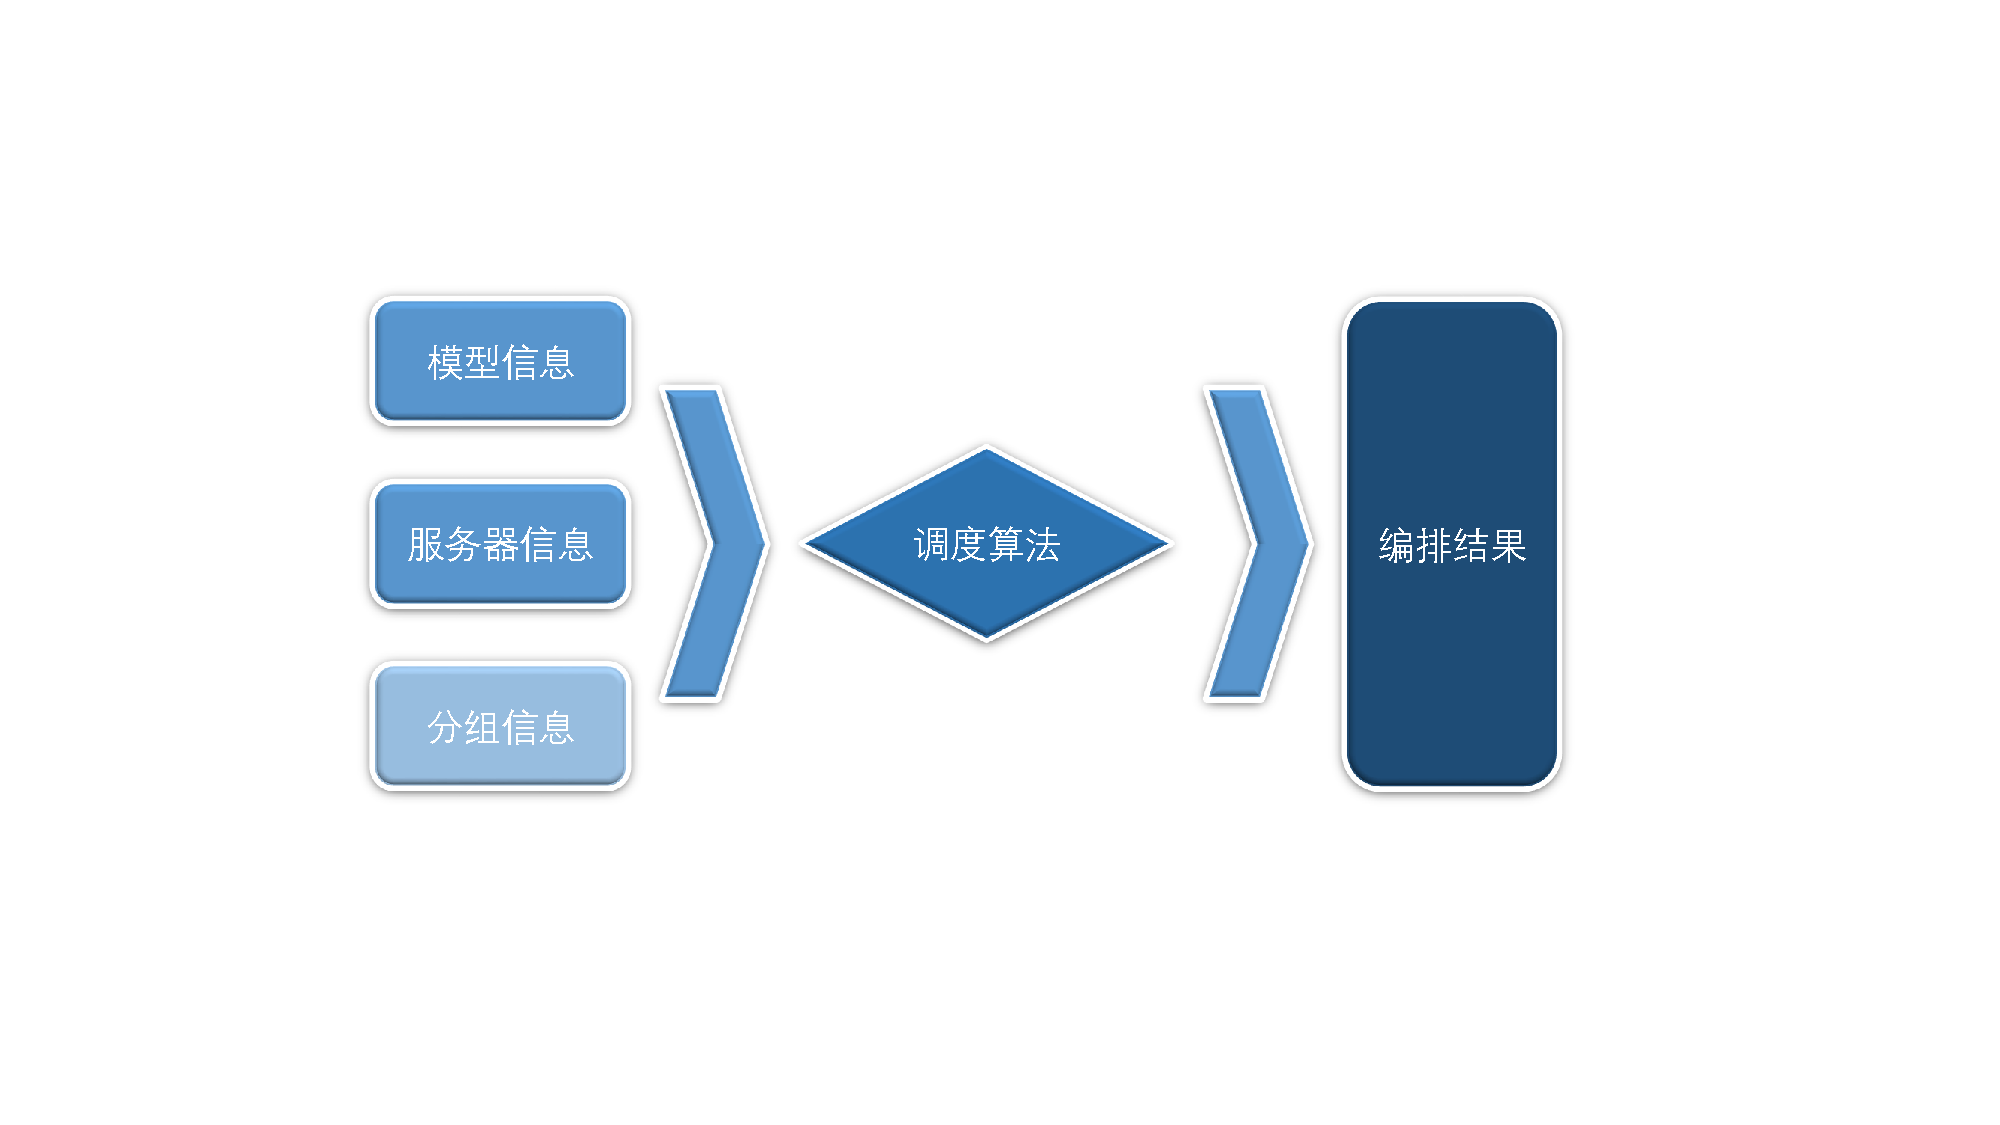
\includegraphics[width=0.8\textwidth]{algo-pic.pdf}

\caption{算法描述}\label{fig:algo}

\end{figure}

\paragraphnl{增量式调度}

我们刚刚描述的算法仅仅完成了从无到有这一步,听起来对于新的业务数据和租户部署来讲,这已经足够了,但是对于一个不能停机,在线上持续提供着服务的集群来讲,这是一个不能接受的逻辑。如果一个不大的变更导致算法重算所有调度结果,使大面积的重分配发生,大量逻辑集群上线与下线发生,服务质量的下降是一个不可接受的事情。因此这里我们需要做一些额外的考虑,避免此类情形发生。为了解决这个问题,我们提出以下三点。

\paragraphnl{一、降低调度算法的重调度率}

对于我们的调度纯函数来讲,增量调度就等于上一次调度输入加上增量补丁后的全部数据再输入调度算法。所以逻辑上不存在“重调度”这个概念。对于重调度的场景,我们可以定义为,两个相差较小的输入各自输出的调度结果的差异。那么这个场景下,我们期望这个差异较小,最好不在边缘数据上有突变。为了达到这个目的,我们可以设法使输入变化时,算法考虑各个模型的顺序变动最少,为了达到这个目的,可以以某种顺序为模型输入排序,也可以要求用户输入额外的数据。

\paragraphnl{二、使用独立的增量调度算法}

kubernetes operator 事实上对于已存在的 CRD 进行变更,变动前后的输入都能获取,这在工程上可以用一些方法实现。对于一个已经初始调度完成的集群,我们的增量调度使用一个独立的算法去完成即可。这里我们可以将变动的每一步拆分开,每一步都进行安全且原子的操作。这里本人暂时没有给出合理的实现,就只提一些思路,不明确描述了。

% TODO: thoughts

\paragraphnl{三、调度逻辑保证服务持续性}

在我们的设计中,算法输出和调度执行拆分为了明确的两个模块,那么我们的执行模块在进行变动时,能进行感知,并且做出考虑,比如在新的部署就绪之前,不下线旧的部署,这样就可以保证服务质量。当然这里有一些其他细节问题,我们就不陷入工程细节,赘述了。

% TODO: rearrange rate

\subsection{效果对比}

本部分我们将人工编排的部署方式,不在服务器重叠多个业务租户,或者小规模的情况下将所有业务租户重叠部署在所有服务器上的情况,和我们的算法给出的结果进行对比。值得注意的是,这里在给定资源和要求的前提下,算法输出可以按照算法模块的输出即可,与执行器的动作无关。我们的对比也仅仅是理论计算为主。对于涉及执行的部分则不能如此。例如实际执行压力测试,观察效果。

\subsubsection{结果举例}

本部分列出几个调度输入以及对应的输出。

\begin{table}[]
\begin{tabular}{llll}
输入 & 模型名     & 内存    & 计算资源  \\
   & mnist   & 100   & 50    \\
   & dummy   & 50    & 10    \\
   & 服务器副本数  & 内存    & 计算资源  \\
   & 1       & 1024  & 200   \\
输出 & pod 副本数 & 模型名   &       \\
   & 1       & mnist & dummy
\end{tabular}
\caption{简单输入}
\end{table}

\begin{table}[]
\begin{tabular}{llll}
输入 & 模型名      & 内存    & 计算资源     \\
   & mnist    & 100   & 50       \\
   & dummy    & 50    & 10       \\
   & big\_cnn & 500   & 200      \\
   & 服务器副本数   & 内存    & 计算资源     \\
   & 1        & 200   & 100      \\
   & 1        & 600   & 300      \\
输出 & pod 副本数  & 模型名   &          \\
   & 1        & mnist & big\_cnn \\
   & 1        & dummy &
\end{tabular}
\caption{复杂输入 - 多个 Deployment 输出}
\end{table}

\begin{table}[]
\begin{tabular}{llll}
输入 & 模型名     & 内存            & 计算资源  \\
   & mnist   & 100           & 50    \\
   & dummy   & 50            & 10    \\
   & test1   & 200           &       \\
   & test2   & 180           &       \\
   & test3   & 210           &       \\
   & 分组      & 模型名           & 计算资源  \\
   &         & test\{1,2,3\} & 200   \\
   & 服务器副本数  & 内存            & 计算资源  \\
   & 2       & 600           & 200   \\
输出 & pod 副本数 & 模型名           &       \\
   & 1       & mnist         & dummy \\
   & 1       & test\{1,2,3\} &
\end{tabular}
\caption{分组输入 - 指定模型组总计算资源消耗}
\end{table}

% \subsubsection{资源利用率}

% 本部分对比在人工部署,逻辑集群上不堆叠多个业务时,资源利用率和我们的方法相比如何。

\subsubsection{容灾能力}

本部分测试在一些节点随机失效的前提下,系统是否能够继续提供服务,照常工作。对于基于 kubernetes 的调度编排系统来说,测试环境的 pod 可以看作大规模部署下的服务器,我们随机 kill 一定比例的 pod 就可以模拟服务器故障的场景。对于传统运行方式,则可以通过 kill 服务进程的方式来模拟。

我们测试了 kill 在运行的进程,可见容器在30秒之内均能被重新启动,可见 kubelet 的原地进程监控与重启直接保证了容灾能力。但是崩溃的过程中,过少的 pod 数量将会导致服务能力不足,导致部分请求不能被响应,延迟提高等后果。这仍然需要部署时计算好足够的计算资源数再提交任务。

\subsubsection{性能测试与压力测试}

本部分测试整个系统的抗压能力,不止是算法的理论推导部分。我们的测试方法是采用 grpc 客户端去请求 Tensorflow Serving 服务,加大压力观察服务的承载能力。这个测试一方面可以对比两种部署方式的承载能力,给出结论,另一方面也可以证明本设计的系统确实可以工作,并且有工业级的能力。

我们预期两种方式的性能差距很小,如果有差距,可能来源于资源限制或者 kubernetes 的 proxy 和网络组件造成的 overhead。
